\documentclass[12pt]{article} % use larger type; default would be 10pt
\usepackage[czech]{babel}
\usepackage[utf8]{inputenc} % set input encoding (not needed with XeLaTeX)

%%% PAGE DIMENSIONS
\usepackage{geometry} % to change the page dimensions
% \usepackage[left=2cm,right=2cm,top=2cm,bottom=2cm]{geometry}
\geometry{a4paper}
% \geometry{margin=2in} % for example, change the margins to 2 inches all round
% \geometry{landscape} % set up the page for landscape

\usepackage{graphicx} % support the \includegraphics command and options
\usepackage{wrapfig} % support the wrapfigure section

\usepackage{hyperref} % links in \tableofcontents
\hypersetup{
	colorlinks,
	citecolor=black,
	filecolor=black,
	linkcolor=black,
	urlcolor=black
}

% \usepackage[parfill]{parskip} % Activate to begin paragraphs with an empty line rather than an indent

%%% PACKAGES
\usepackage{booktabs} % for much better looking tables
\usepackage{array} % for better arrays (eg matrices) in maths
%\usepackage{paralist} % very flexible & customisable lists (eg. enumerate/itemize, etc.)
\usepackage{verbatim} % adds environment for commenting out blocks of text & for better verbatim
\usepackage{subfig} % make it possible to include more than one captioned figure/table in a single float
% These packages are all incorporated in the memoir class to one degree or another...
\usepackage{tikz} % graphs
\usepackage{pgfplots}
\usepackage{float}

%%% HEADERS & FOOTERS
\usepackage{fancyhdr} % This should be set AFTER setting up the page geometry
\pagestyle{fancy} % options: empty , plain , fancy
\renewcommand{\headrulewidth}{0pt} % customise the layout...
\lhead{}\chead{}\rhead{}
\lfoot{}\cfoot{\thepage}\rfoot{}

%%% SECTION TITLE APPEARANCE
\usepackage{sectsty}
\allsectionsfont{\sffamily\mdseries\upshape} % (See the fntguide.pdf for font help)
% (This matches ConTeXt defaults)

%%% ToC (table of contents) APPEARANCE
\usepackage[nottoc,notlof,notlot]{tocbibind} % Put the bibliography in the ToC
\usepackage[titles,subfigure]{tocloft} % Alter the style of the Table of Contents
\renewcommand{\cftsecfont}{\rmfamily\mdseries\upshape}
\renewcommand{\cftsecpagefont}{\rmfamily\mdseries\upshape} % No bold!
\newcommand{\bigsize}{\fontsize{35pt}{20pt}\selectfont}

%%% END Article customizations

\begin{document}
\begin{titlepage}
	
\includegraphics[scale=0.7]{logo.jpg}
	\vspace*{\fill}
	\begin{center}
		\textsc{\LARGE Operační zesilovač II}\\[1cm]
		Martin Zlámal \\[1cm]
		{\small\em \ Datum měření 27. března 2014 } \\
		{\small\em \copyright \ Datum poslední revize \today } \\
		\LaTeX
	\end{center}
	\vspace*{\fill}
\end{titlepage}
%\tableofcontents
%\listoffigures
%\listoftables
\newpage

\section{Zadání}
Změřte postupně statickou převodní charakteristiku invertujícího, neinvertujícího 
zapojení a komparátoru s monolitickým operačním zesilovačem (OZ). Měření proveďte pro 
různá zesílení a změřené charakteristiky vyneste do grafů.

\section{Schémata zapojení}
\begin{figure}[H]
\center
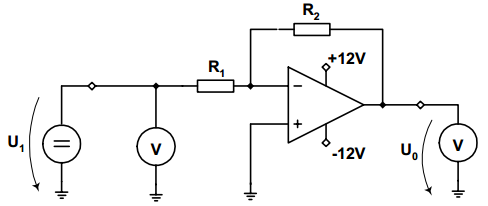
\includegraphics[scale=0.7]{schema1.png}
\caption{Operační zesilovač v invertujícím zapojení}
\end{figure}

\begin{figure}[H]
\center
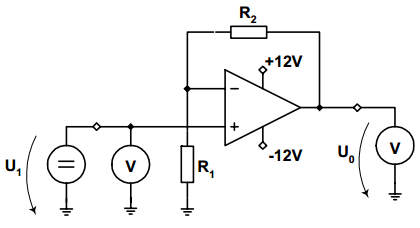
\includegraphics[scale=0.7]{schema2.png}
\caption{Operační zesilovač v neinvertujícím zapojení}
\end{figure}

\begin{figure}[H]
\center
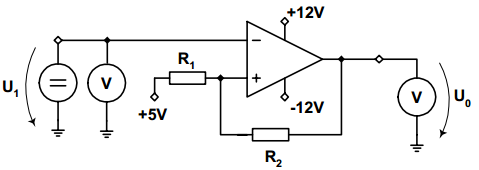
\includegraphics[scale=0.7]{schema3.png}
\caption{Operační zesilovač jako komparátor s hysterezí}
\end{figure}

\section{Naměřené a vypočítané hodnoty}
Pro měření operačních zesilovačů volíme napájení $\pm12\,V$. Pro invertující zapojení OZ volíme hodnoty rezistorů $R_1=10\,k\Omega$ a $R_2=20\,k\Omega$ tak, aby bylo zesílení $A_U=-2$ podle následujícího vztahu.
\begin{equation}
A_U = -\frac{R_2}{R_1}=-\frac{20k}{10k}=-2
\end{equation}

\begin{table}[H]
\center
\caption{Převodní charakteristika invertujícího OZ, kladná polarita}
\begin{tabular}{|c|c|c|c|c|c|c|c|}
\hline 
$U_1\,[V]$ & 0,98 & 1,95 & 2,93 & 3,90 & 4,89 & 5,88 & 6,86 \\ 
\hline 
$U_0\,[V]$ & -1,96 & -3,90 & -5,86 & -7,82 & -9,76 & -9,92 & -9,92 \\ 
\hline 
\end{tabular}
\end{table}

\begin{table}[H]
\center
\caption{Převodní charakteristika invertujícího OZ, záporná polarita}
\begin{tabular}{|c|c|c|c|c|c|c|c|}
\hline 
$U_1\,[V]$ & -1,01 & -2,00 & -2,99 & -3,98 & -4,97 & -5,96 & -6,95 \\ 
\hline 
$U_0\,[V]$ & 2,01 & 3,99 & 5,97 & 7,95 & 9,93 & 11,20 & 11,20 \\ 
\hline 
\end{tabular}
\end{table}

Pro neinvertující zapojení OZ volíme hodnoty rezistorů $R_1=10\,k\Omega$ a $R_2=100\,k\Omega$ tak, aby bylo zesílení $A_U=11$ podle následujícího vztahu.
\begin{equation}
A_U = \frac{R_2}{R_1}+1=\frac{100k}{10k}+1=11
\end{equation}

\begin{table}[H]
\center
\caption{Převodní charakteristika neinvertujícího OZ, pouze kladná polarita}
\begin{tabular}{|c|c|c|c|c|c|c|c|c|c|c|c|}
\hline 
$U_1\,[V]$ & 0,1 & 0,2 & 0,3 & 0,4 & 0,5 & 0,6 & 0,7 & 0,8 & 0,9 & 1,0 & 2,0 \\ 
\hline 
$U_0\,[V]$ & 1,26 & 2,13 & 3,46 & 4,46 & 5,51 & 6,62 & 7,77 & 8,83 & 9,90 & 11,20 & 11,27 \\ 
\hline 
\end{tabular}
\end{table}

Pro komparátor s hysterezí volíme hodnotu rezistorů $R_1=10\,k\Omega$ a $R_2=100\,k\Omega$ tak, aby šířka hysterezního pásma přibližne $U_H=2\,V$ podle následujícího vztahu.
\begin{equation}
U_H \approx 2\cdot U_{SAT}\cdot \frac{R_1}{R_1+R_2}=2\cdot 10\cdot \frac{10k}{10k+100k}\doteq 1,82
\end{equation}

\begin{table}[H]
\center
\caption{Převodní charakteristika komparátoru}
\begin{tabular}{|c|c|c|c|c||c|c|c|c|c|}
\hline 
$U_1\,[V]$ & 2,30 & 5,59 & 5,6 & 7,00 & 7,00 & 3,72 & 3,71 & 2,30 \\ 
\hline 
$U_0\,[V]$ & 11,28 & 11,28 & -9,95 & -9,95 & -9,95 & -9,95 & 11,28 & 11,28 \\ 
\hline
\end{tabular} 
\end{table}

\section{Grafy}
\begin{figure}[H]
\centering
	\begin{tikzpicture}
		\begin{axis}[
			width=1\textwidth,
	     	height=0.5\textwidth,
			xlabel={$U_1\,[V]$},
			ylabel={$U_0\,[V]$},
			grid=major,
			minor tick num=3,
			axis y line=center,
			axis x line=middle
		]
		\addplot coordinates {
			(-6.95,11.2)
			(-5.96,11.2)
			(-4.97,9.93)
			(-3.98,7.95)
			(-2.99,5.97)
			(-2.00,3.99)
			(-1.01,2.02)
			(0.98,-1.96)
			(1.95,-3.90)
			(2.93,-5.86)
			(3.90,-7.82)
			(4.89,-9.76)
			(5.88,-9.92)
			(6.86,-9.92)
		};
%		\addlegendentry{...}
		\end{axis}
	\end{tikzpicture}
	\caption{Převodní charakteristika invertujícího zapojení OZ}
\end{figure}

\begin{figure}[H]
\centering
	\begin{tikzpicture}
		\begin{axis}[
			width=1\textwidth,
	     	height=0.5\textwidth,
			xlabel={$U_1\,[V]$},
			ylabel={$U_0\,[V]$},
			grid=major,
			minor tick num=3,
			axis y line=center,
			axis x line=middle
		]
		\addplot coordinates {
			(0.1,1.26)
			(0.2,2.13)
			(0.3,3.46)
			(0.4,4.46)
			(0.5,5.51)
			(0.6,6.62)
			(0.7,7.77)
			(0.8,8.83)
			(0.9,9.90)
			(1.0,11.12)
			(2.0,11.27)
		};
%		\addlegendentry{...}
		\end{axis}
	\end{tikzpicture}
	\caption{Převodní charakteristika neinvertujícího zapojení OZ}
\end{figure}

\begin{figure}[H]
\centering
	\begin{tikzpicture}
		\begin{axis}[
			width=1\textwidth,
	     	height=0.5\textwidth,
			xlabel={$U_1\,[V]$},
			ylabel={$U_0\,[V]$},
			grid=major,
			minor tick num=3,
			axis y line=center,
			axis x line=middle
		]
		\addplot coordinates {
			(2.30,11.28)
			(5.59,11.28)
			(5.60,-9.95)
			(7.00,-9.95)
		};
		\addlegendentry{zvyšování napětí $U_1$}
		\addplot coordinates {
			(7.00,-9.95)
			(3.72,-9.59)
			(3.71,11.28)
			(2.30,11.28)
		};
		\addlegendentry{sninžování napětí $U_1$}
		\end{axis}
	\end{tikzpicture}
	\caption{Převodní charakteristika komparátoru}
\end{figure}

\section{Závěr}
Z grafu pro invertující zapojení OZ je vidět, že čím je menší napětí $U_1$, tím je větší výstupní napětí $U_0$ (a obráceně) a to až do saturačního napětí $U_{SAT}$, které je pro obě polarity $U_1$ z hlediska velikosti rozdílné.

Oproti tomu neinvertující zapojení má kladné zesílení $A_U$, ale mnohem větší ($A_U=11$). Tzn., že saturace dosáhneme již při hodnotě $U_1\approx 1\,V$.

Jak je vidět, tak hysterezní smyčka není přesně souměrná kolem hodnoty $U_1=5\,V$ viz schéma zapojení. To je způsobeno nepřesnou volbou saturačního napětí $U_{SAT}$ do výpočtu šířky hysterezního pásma. Každopádně samotný výsledek tento fakt nijak neovlivňuje.

\end{document}
